% ----------------------------------------------------------
\chapter{Theoretical Background}
\label{theoretical_background}
% ----------------------------------------------------------

This chapter presents the theoretical background for the technologies and ideas discussed in this work. It explores two distinct but connected areas. Firstly, it examines ITS applications and the challenges faced in the field. Secondly, it provides an overview of some sensors, and their role in autonomous vehicles technologies. In addition, the chapter contextualizes the areas of sensor fusion in relation to traffic monitoring and cooperative perception. Finally, the simulation environment used for the research experiments is presented.

% ---
\section{Intelligent Transportation Systems}
% ---

Intelligent Transportation Systems (ITS) are a collection of applications that utilize information and communication technologies to optimize various aspects of transportation and traffic management \cite{chen2022constructing}. The goal is to promote safer, more efficient, and coordinated usage of transport networks, with a primary focus on road transport. 

This includes infrastructure, vehicles, and users, as well as traffic and mobility management systems. These systems include a wide range of technologies, from basic navigation aids and traffic signal controls to advanced applications that integrate real-time data from various sources, such as weather updates, parking guidance systems, and predictive modeling tools. 

% The deployment of ITS aims to increase road capacity, reduce travel times, and enhance safety measures. However, it is important to consider privacy and surveillance implications caused by this. This kind of data can present a real privacy risk if data life cicle is not correctly managed.

Emerging technologies, such as smart cities and the Internet of Things, have driven the emergence of Intelligent Transportation Systems \cite{qureshi2013survey}. Large cities are investing in the necessary data infrastructure to support this new paradigm. However, the placement of embedded devices in the infrastructure presents challenges in terms of deployment and maintenance costs \cite{s18041212}.

ITS applications have used various data sources, such as smart cards, Radio Frequency Identification (RFID) tags, sensors, video cameras, Global Positioning Systems (GPS), social media and high-definition (HD) maps \cite{bhatia2022intelligent}. In this context, Autonomous Vehicles (AVs) are seen as an attractive technology in which data generated from sensors can be reused for the input of sophisticated algorithms that feed ITS applications.

\begin{figure*} [!ht]
    \centering
    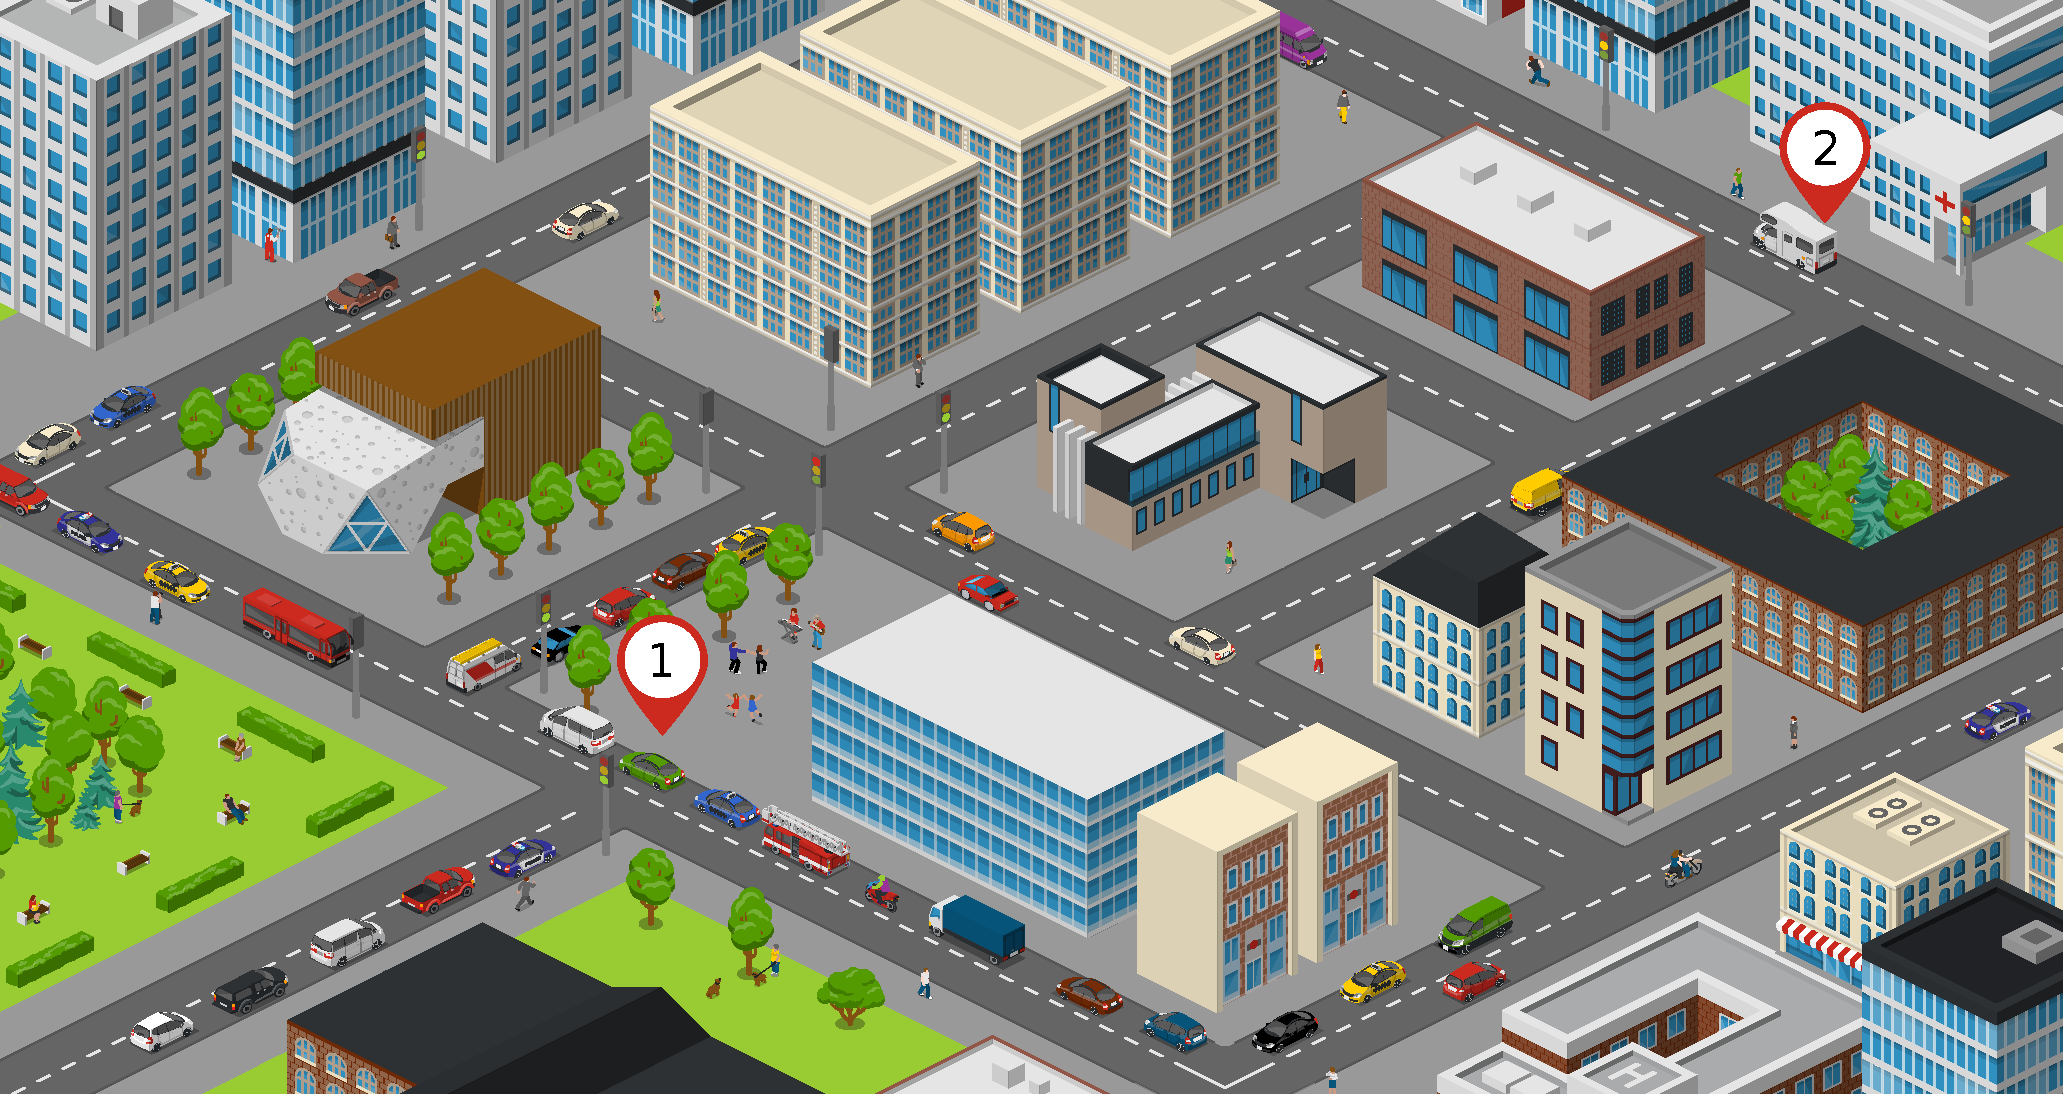
\includegraphics[width=1\textwidth]{parts/figuras/virtual-its-v2.pdf}
    \caption{1 represents a busy street with traffic lights and cameras, 2 is a less busy street that contains no road sensing infrastructure.}
    \label{fig:virtual_its_infrastructure}
\end{figure*}

Figure \ref{fig:virtual_its_infrastructure} shows an example of an application scenario. A busy street (1) contains several sensors on traffic lights, RSUs and other systems integrated to the road infrastructure. A less busy street can be observed in 2. On this street, it is possible to take advantage of the vehicles sensors to complement existing information that existing infrastructure sensors can't provide. Also, with shared data on the other roads, a driver or an autonomous vehicle can make smart detour decisions to avoid traffic jams.

With a data service that could provide real time data of only position and speed, ITS technology can offer, among other things: traffic monitoring and forecasting even in locations where there are no stationary traffic sensing units.

% ---
\section{Autonomous vehicles and sensors}\label{av-sensors}
% ---

According to the Society of Automotive Engineers (SAE International) J3016 standard, there are six levels of driving automation, from  “no automation” to “full automation” and they are summarized in table \ref{tab-levels}.

\begin{table}[htb]
\footnotesize
\begin{tabular}{|p{1.0cm}|p{3.0cm}|p{3.5cm}|p{3.3cm}|p{3.3cm}|}
   \hline
   \textbf{Level} & \textbf{Name}  & \textbf{Steering and Acceleration/Deceleration}  & \textbf{Monitoring of Environment}  & \textbf{Dynamic Driving Task} \\
    \hline
    0 & No Automation  & Human driver & Human driver  & Human driver \\
    \hline
    1 & Driver Assistance & Human driver and System & Human driver & human driver \\
    \hline
    2 & Partial Automation & System & Human driver & Human driver \\
    \hline
    3 & Conditional Automation & System & System & Human driver \\
    \hline
    4 & High Automation & System & System & System \\
    \hline
    5 & Full Automation & System & System & System \\
    \hline
\end{tabular}
\caption{J3016 levels of driving automation}
\label{tab-levels}
\end{table}

The more automated the system in table \ref{tab-levels}, the more reliant it becomes to sensor data. State-of-the-art AVs utilize a wide range of on-board sensors. High sensor redundancy is required for robustness and reliability in most of the vehicle tasks \cite{9046805}. Electric vehicles have and increasing number of sensors, as reference data points, the BYD Atto 3 has 5 cameras and the Tesla Model 3 has 9.

Sensor data provides critical information about the environment, the driving area, and potential obstacles in the vehicle path. The data collected by these sensors forms the basis for the autonomous vehicle's decision-making and control systems \cite{li2023learning}.

The different modalities of sensors address different aspects of environmental perception. For example, cameras are adept at sensing color without emitting signals for measurement, making them valuable for tasks such as traffic light detection. However, they are sensitive to changes in illumination and have limitations in obtaining depth information. 

Lidar and radar sensors, on the other hand, excel at measuring depth and distance to objects, providing critical 3D information that complements the data captured by cameras. Ultrasonic sensors, with their ability to detect obstacles and measure distance using sound waves, further enhance the sensor suite of autonomous vehicles.

% ---
\section{Simultaneous Localization and Mapping}
% ---

Simultaneous Localization and Mapping (SLAM) is a set of methods and algorithms that find vehicle location in a space reference frame while simultaneously mapping the given surrounding space \cite{Zheng2023}. This is critical to navigate and operate in unknown or dynamic environments, specially if existing maps or external localization systems are unavailable or connection is unstable.

SLAM combines sensor data, such as visual, inertial, and depth information. With this data it is possible to estimate the vehicle's pose and location and construct an updated map of the environment in real time. Using the self-generated map and continuous localization estimates, robotic systems can plan and execute trajectories, avoid obstacles, and interact with their environment in a robust and autonomous manner.

SLAM is critical for cooperative perception, as any shared perception message will contain location information of the vehicle and the perceived surrounding. If the vehicle location is imprecise, this will impact the localization of any detected objects.

Considering that Localization is the task to position the car relative to a reference frame in the environment, by having this shared reference frame, its possible to combine data from several different vehicles and apply that to a shared localization and mapping application.

%State of the art SLAM techniques can be categorized in several ways, one could categorize they by the used algorithms like Filter Based SLAM or Deep Learning Based SLAM.
When looking to State of the art SLAM techniques from the sensor point of view, they can be split in 3 types: visual SLAM, lidar SLAM, and multi-sensor SLAM. A recent SOTA comparison in \cite{garigipati2022} found that overall, Lidar-based methods generally outperformed visual SLAM in outdoor settings and with dynamic objects, benefiting from their broader field of view.

% ---
\section{Sensors}
% ---

The main types of sensor devices used for perception in the context of autonomous vehicles are described in the following subsections. 

% ---
\subsection{Radar}
% ---

Radar technology, short for Radio Detection and Ranging, is a detection system that uses radio waves to determine the range, angle, or velocity of objects. It was initially developed for military purposes prior to World War II. Radar systems can detect ships, missiles, vehicles, aircraft, and other objects by sending out pulses of high-frequency electromagnetic waves and observing the echoes that are returned. One of the advantages of this sensor is that velocity and position can be measured simultaneously based on the Doppler Effect.

In present days radar technology found a big number of applications, relevant examples for this work are: air traffic control, weather forecasting, traffic monitoring and autonomous vehicles. When used on autonomous vehicles, radar provides real-time data for obstacle detection, speed measurement, and collision avoidance. It can operate in various light conditions and can complement other sensors such as LiDAR and cameras to enhance vehicle perception systems.

Current standard frequency for Autonomous Vehicles by the European Telecommunications Standards Institute is between 77 and 81 GHz (ETSI TR 103 593 and \cite{ramasubramanian2018moving}). These frequencies are fast enough to provide the reaction time required by autonomous vehicles and are accurate up to a distance of 250 meters.

Notable radar limitations include susceptibility to jamming and electromagnetic interference, multiple Reflections and Clutter. Clutter refers to unwanted echoes or signals detected by radar systems from objects that are not the target of interest. These may include reflections from the ground, buildings, trees, and other static objects, as well as atmospheric phenomena such as rain and snow.

For comprehensive awareness, autonomous vehicles typically have six to ten radar sensors placed around them (with an exception in Tesla vehicles). In 2022, Waymo's self-driving taxi had six radar sensors, while Mercedes-Benz used eight radar sensors in their test vehicles.

% ---
\subsection{LiDAR}
% ---

LiDAR is an acronym for Light Detection and Ranging, it is a remote sensing method that uses light in the form of a pulsed laser to measure the distance between objects. The system determines the distance to an object by emitting light pulses and measuring the time it takes for the reflected pulses to return. 

This technology was initially developed in the 1960s, shortly after the invention of the laser. It was first used in military research (for satellite tracking) and meteorological tasks, like measuring clouds and pollution.

LiDAR has been applied across diverse fields over the years, besides autonomous vehicles, it has a big number of applications. Relevant recent usages are astronomy (Mars topology analysis and Navigation Doppler Lidar), Archaeology (Upano Valley sites) and Military.

The current state of technology employed in autonomous vehicles allows for a range of up to 400 meters. The sensor outputs the position and intensity of light reflected at a given point, allowing for the measurement of both distance and reflectance values. This information can be used to create a 3D point cloud of the vehicle's surroundings.

LiDAR is a significant component alongside cameras and radars and is favored for its precision in range measurement, which is crucial for detecting other vehicles, pedestrians, and various entities to ensure more safe traffic \cite{li2020lidar}.

In the literature, the biggest limitations of this kind of sensor are high costs, big volume of generated data management and bad performance with adverse surface types or under bad weather condition \cite{s23062972}.

% ---
\subsection{Cameras}
% ---

Digital camera technology is designed to capture optical images using photosensitive sensors to convert light into electronic signals that form digital images. Cameras operate by focusing light through a lens onto a sensor array that records the light intensity and color of the 3D space into a projected 2D image.

An image sensor array typically consists of a CCD (Charge-Coupled Device) or CMOS (Complementary Metal-Oxide-Semiconductor) image sensor. These two types of image sensors are widely used in camera technology. CCD sensors are preferred for applications where image clarity and detail are the priority, such as in astrophotography and high-end digital photography, due to their high-quality images and better light sensitivity.

On the other hand, CMOS sensors have a construction that enables independent reading of each pixel. This feature contributes to faster processing speeds and lower power consumption compared to CCDs. Therefore, CMOS sensors are particularly attractive for use in devices where battery life and rapid image capture are critical, such as mobile phones and some consumer-grade cameras.

The history of camera technology dates back to the early 1600s with the formal invention of the camera obscura (earlier experiments of the actual technology usage dates back to as far as 500 AD). Since then, significant progress has been made, particularly in digital imaging during the latter part of the 20th century. Initially used for artistic and documentary purposes, cameras quickly found applications in various fields, including science, security, entertainment, and more recently, in autonomous vehicle systems.

Compared to other sensors, cameras have very distinct features. They work for long and short range detection and have large field of vision and angular resolution. The cost can be high, in case advanced camera sensors with high resolution are being used, but can also be very low if simpler settings are used, especially when compared with LiDAR sensors.

Despite being critical components, cameras come with several limitations that can impact their performance and reliability, a few examples are: sensitivity to environmental conditions, like fog, heavy rain and night; limitations in perceiving depth; difficulties with direct sunlight and high lighting variations.

In autonomous vehicles, digital images provide visual information about the vehicle surroundings that other sensors cannot capture, like information from traffic lights or traffic signs. In recent years Tesla moved to a new program called Tesla Vision, in which it replaced radar and ultrasonic sensors by camera sensing, believing that the future in AV sensing is in image\footnote{https://www.tesla.com/support/transitioning-tesla-vision}.

As reference, we observe that new electric vehicles come equipped with an increasing number of cameras, the BYD Atto 3 has 5 cameras and the Tesla Model Y currently has 9\footnote{https://www.tesla.com/ownersmanual/modely/en\_us/GUID-682FF4A7-D083-4C95-925A-5EE3752F4865.html}.

% ---
\subsection{GNSS}
% ---

GNSS (Global Navigation Satellite System), commonly referred to as GPS (Global Positioning System), is a satellite-based navigation system that provides geolocation information to a receiver anywhere on the planet. GPS refers to the North American Global Positioning System, while GNSS refers to the International Multi-Constellation Satellite System. This means that it has access to other satellite systems, such as GLONASS, Baidu, Galileo, and others, in addition to GPS.

Initially developed by the United States Department of Defense in the 1970s, the technology was intended for military navigation. Since then, it has expanded vastly in its applications across various sectors.

The sensor system operates by using a network of satellites that transmit radio signals to receivers on the Earth's surface. These signals provide data on the satellites' location and the exact time the signals were transmitted. The GNSS receiver calculates its own position by measuring the time delay between receiving the signals from at least four satellites. This time delay helps determine the distance from each satellite. By determining the distance to multiple satellites, the receiver can triangulate its position in three dimensions.

Recent advancements have improved the accuracy of GNSS technology in civilian use to within a few meters. In autonomous vehicles, GNSS provides critical positioning data that supports other sensors, such as cameras and LiDAR, to create a comprehensive understanding of the vehicle's environment.

GNSS systems face challenges such as signal disruption or blockage in closed or dense environments, as well as vulnerability to signal interference and spoofing. While GNSS provides global coverage and has broad applications, these challenges can limit its reliability and performance in critical navigation and timing tasks.

% ---
\subsection{IMU}
% ---

Inertial Measurement Unit (IMU) sensing consists of a combinations of accelerometers, gyroscopes, and magnetometers that provide data used to track an object's acceleration, rotational motion, and orientation. IMU technology is currently used in a wide range of applications, including navigation systems, consumer electronics, robotics, and also in the field of autonomous vehicles. 

IMUs have an important role in autonomous vehicles by providing essential data for dead reckoning and improving the vehicle's ability to determine its position and orientation in situations where GNSS may be unreliable or unavailable, such as tunnels or urban canyons.

The sensor nature enables integration with other systems, such as GNSS, LiDAR, and radar, forming a comprehensive sensory network that significantly reduces the system's vulnerability to the failure of any single sensor.

However, this kind of sensor also have its limitations. Notable challenge are temperature sensitivity and drift errors in accelerometer and gyroscope readings, which can accumulate over time and lead to increasing inaccuracies if not regularly corrected or calibrated.

Not all autonomous vehicles use IMUs. For example, Waymo does not employ this sensor on their autonomous vehicles. Instead, they use a combination of LiDAR, radar, and cameras.

% ---
\section{Cooperative perception}\label{cooperative-perception}
% ---

In an abstract view, cooperative perception can be seen as the collaborative exchange and integration of data among system components to enhance their overall situational awareness beyond individual capabilities.

The concept has derived from research in vehicle-to-vehicle (V2V) and vehicle-to-infrastructure (V2I) communications. The shared perception approach allows robots and autonomous vehicles to collectively perceive and interpret environment data, significantly increasing the accuracy and reliability of the information derived when compared to isolated systems which rely solely on onboard sensors \cite{YU2022100023}.

Although cooperative perception technology has promising benefits, it also faces significant limitations. High bandwidth and latency requirements are necessary due to the real-time sharing of data among multiple entities. Furthermore, challenges such as data privacy, security, and integration of heterogeneous systems are ongoing fields of research. The effectiveness of the technology is limited in areas with poor network coverage or compromised network infrastructure due to its dependence on consistent connectivity.

The current SOTA methods in cooperative perception technology seek to address these limitations by optimizing data transmission mechanisms\cite{THANDAVARAYAN2023103655} and integrating machine learning algorithms to enhance data processing efficiency and accuracy \cite{xu2022v2xvit}.

Intelligent Transportation Systems (ITS) can integrate these advancements in cooperative perception technology to create more efficient, safer, and more responsive transportation networks. Through ITS, vehicles can communicate with each other and with traffic management systems, resulting in improved traffic flow, reduced congestion, and enhanced safety.

The use of cooperative perception in ITS is relevant because it enables a shared situational awareness. This awareness allows proactive traffic management and incident response strategies not only on the personal level for the vehicle but for the road infrastructure as a whole.

% ---
\section{Sensor fusion for ITS applications}\label{sensor-fusion-its}
% ---

In the same sense as cooperative perception, but at a lower level, sensor fusion is a method where data from various sources is combined to enhance individual measurements.

Current state of the art research on multi-sensor fusion systems for Autonomous Vehicles have a prevalence of three kinds of combinations in the literature: camera-LiDAR(CL), camera-radar(CR) and camera-LiDAR-radar(CLR).

Data fusion approaches can be categorized based on the abstraction level at which sensor data is integrated. According to \cite{s21062140}, when thinking about multi sensor data fusion, there are three primary data fusion classifications used in modern sensor systems: High-Level Fusion(HLF), Mid-Level Fusion(MLF), and Low-Level Fusion(LLF).

LLF is the most granular approach, also known as data level fusion, it consists of combining raw data from all sensors directly. This method is ideal for applications requiring high precision and extensive data detail, as it preserves all of the original sensor information. While it increases the potential accuracy and robustness of sensor interpretations, it also significantly increases the complexity of data processing and requires sophisticated calibration and alignment of sensors. It also generates a large volume of data that can be difficult to manage and process effectively.

MLF, also referred to as feature-level fusion, integrates data by extracting features from individual sensor data before combining them. This method balances between integrating raw data and processed results,  providing a moderate level of detail and processing complexity. It allows for better context retention than HLF by using raw data’s features rather than completely processed data. However, MLF requires large training sets for effective feature selection and can be challenging to calibrate accurately.

HLF works by first processing data from individual sensors, each of which independently performs detection or tracking algorithms. These results are then combined into a consolidated object definition. The main advantage of this approach is its simplicity, which requires less computation (since it is offloaded to the sensor systems) and less detailed understanding of the underlying sensor technologies. However, HLF can result in the loss of potentially valuable information, as only the processed results from each sensor are merged, discarding any raw data that may contain useful, subtle details.

The nature of sensor fusion presents complex challenges. With the large volume of data from diverse sensors, synchronization becomes imperative to ensure reasonable performance. Given that different sensors emit data at irregular intervals, they are subject to processing delays and transmission latency. If these factors are not properly addressed, they could result in miscommunication or error.

ITS represent a significant area where sensor fusion technology is extensively applied. Sensor fusion for ITS can combine multiple data sources like cameras, radars, and GNSS, to create a more comprehensive understanding of traffic scenarios.

A relevant example is in the context of ITS is Google Maps and Waze, which use data from a large number of users, along with input from mobile phone sensors (which are not necessarily the state of the art in sensing capabilities) and historical traffic data, to predict traffic levels and suggest optimal routes to users. These platforms are simple examples of ITS in action, where sensor fusion can facilitate real-time traffic monitoring and management.

% ---
\section{Simulation environment}\label{sim-env}
% ---


Considering the recent developments in autonomous vehicle technology, researchers need realistic simulations for training and evaluation of AI models and automotive operating systems. The security of V2X systems is also a growing concern, specially in the face of cyber attacks. For these reasons, simulation environments have and important role in analyzing the behavior of communication in V2X systems, and enabling research on topics such as jamming \cite{da2023radio} and spoofing \cite{mullertechnical}. 

Based on this premises, the CARLA simulator and Simu5G were selected for research experimentation. The CARLA simulator is used for physics and environment simulation and the Simu5G is used for network simulations. Both frameworks are open source and extensible, but none was designed with built-in features to integrate with one another. In this sense, a “simulation communication framework” was developed for this work.

Recent research \cite{cislaghi2023simulation} have successfully integrated CARLA and Simu5G by using Message Queues and a controller in each of the services. A similar approach was used and will be further explored in the chapters ahead.

\subsection{CARLA Simulator} \label{carla-sim}

The CARLA simulator, standing for Car Learning to Act \cite{MALIK2022742}, is a platform designed for autonomous driving research and development. It can create controlled and customizable environments for testing autonomous vehicle technologies. CARLA also supports a wide range of scenarios, including weather variations and different traffic conditions. Figure \ref{fig:carla_screenshot} shows an example of the rendered simulation.

\begin{figure*} [!ht]
    \centering
    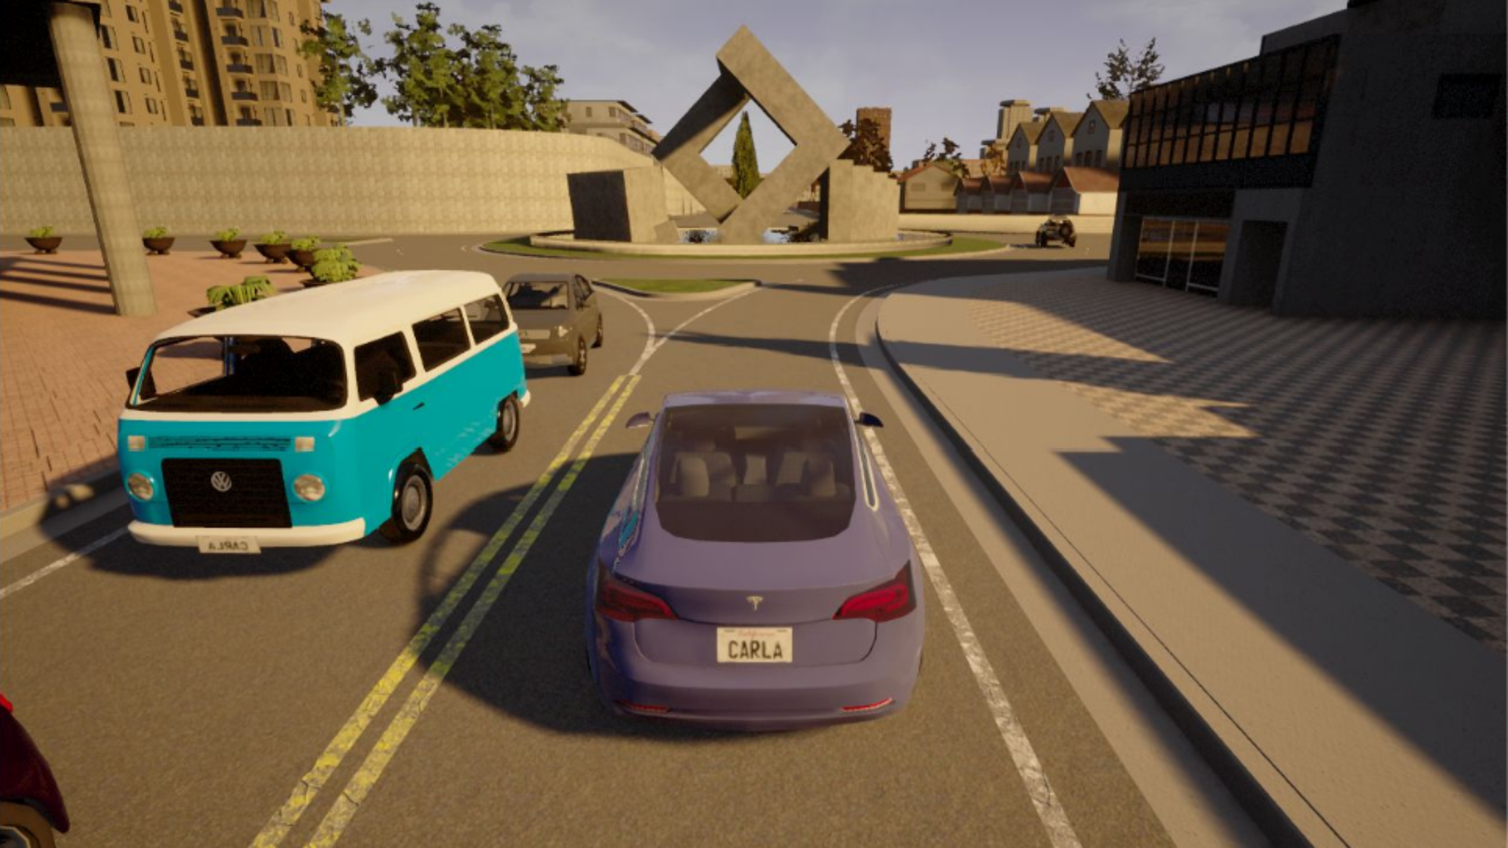
\includegraphics[width=0.80\textwidth]{parts/figuras/carla_screenshot.pdf}
    \caption{A screenshot of a simulation in CARLA. Carla is based on the Unreal Engine 4}
    \label{fig:carla_screenshot}
\end{figure*}

The core motivation for using CARLA is the requirement for risk-free, reproducible, and flexible testing platforms which traditional physical testing methods cannot provide. Its ability to integrate with major machine learning frameworks (as well as ROS robot operating system) and substantial community involvement\footnote{https://github.com/carla-simulator/carla} makes it a reasonable research tool.

\begin{figure*} [!ht]
    \centering
    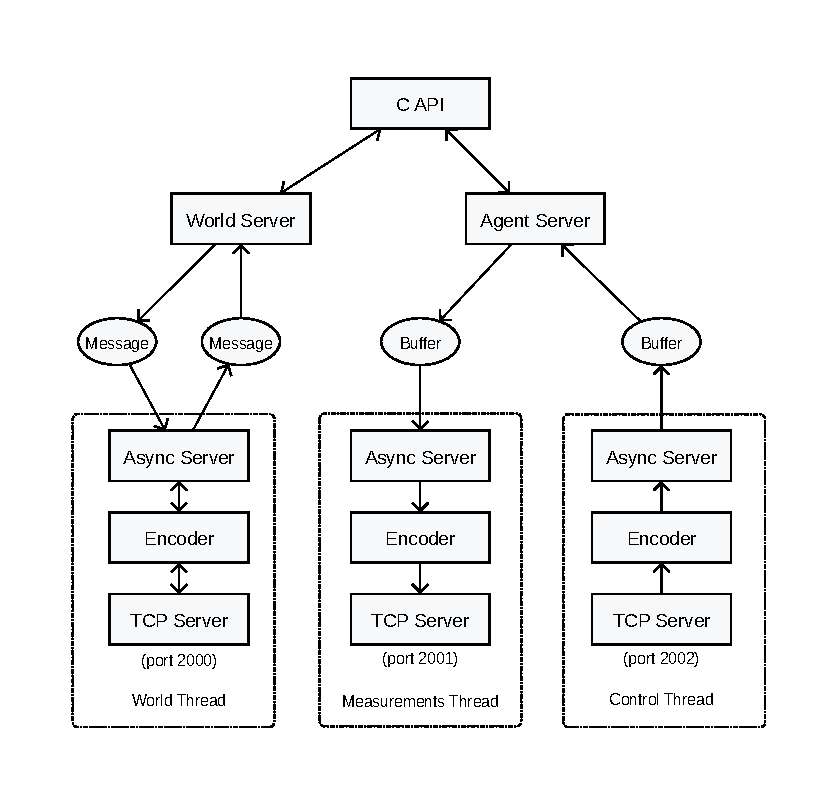
\includegraphics[width=0.70\textwidth]{parts/figuras/carla_architecture.pdf}
    \caption{CARLA architecture, from official documentation https://carla.readthedocs.io/en/stable/carla\_server .}
    \label{fig:carla_architecture}
\end{figure*}

Figure \ref{fig:carla_architecture} depicts the architecture of the CARLA simulator. It is primarily based on a server-client model, with the simulation running as the server and the external control managed by separate client instances. This server can be set up to accept multiple client connections, enabling collaborative testing environments.

The server can be accessed via TCP and has 3 interfaces, the world port, a control port, and the measurements port, each has a server behind which provide a different service.

The "World" server is responsible for controlling the overall simulation environment, while the Agent server has two threads: one dedicated to handling real-time metrics streaming(measurement port) and the other for interactive controls between clients and simulation(control port). This architecture ensures asynchronicity and control even with a considerable number of clients interacting with the server at the same time.

In CARLA, Actors are elements that perform actions within the simulations. These vary from vehicles to pedestrians, each created, managed, and removed through CARLA’s simulated world object, that is accessible within its client API. The essence of the actors lies in their detailed blueprints, which are templates defining attributes like vehicle color, lidar channels, or pedestrian speed. These blueprints are crucial for adding new actors to the simulation as they specify configuration preconditions and spawn behaviors for the Actors.

Finally, at the CARLA environment, sensors serve as the primary medium for data collection and environmental interaction for autonomous systems undergoing testing. A diverse array of sensors is supported, including standard cameras for RGB, depth, and semantic segmentation, GNSS, IMU Lidar and radar. As the sensors simulate real-world device functionality, they facilitate comprehensive testing in a controlled and realistic setting.

\subsection{OMNET++ and Simu5G}

OMNeT++ is an open-source simulation framework designed for network and distributed system simulations. It provides an infrastructure based on components that can be hierarchically nested, allowing researchers to construct the topology of their simulations in a dynamic manner.

The framework supports the implementation of both physical and application-layer network protocols through the use of various modeling techniques, including finite state machines and message passing for communication between components. It contains a graphical interface base on the Eclipse IDE \footnote{https://eclipseide.org/} that can assist in the design, execution, deployment, and analysis of simulation results. Figure \ref{fig:OMNET_IDE} shows an examples of a running experiment at the graphical interface. Network topology is presented at the center of the interface and the network profile is presented below. Network events are displayed sequentially and can be inspected for details.

\begin{figure*} [!ht]
    \centering
    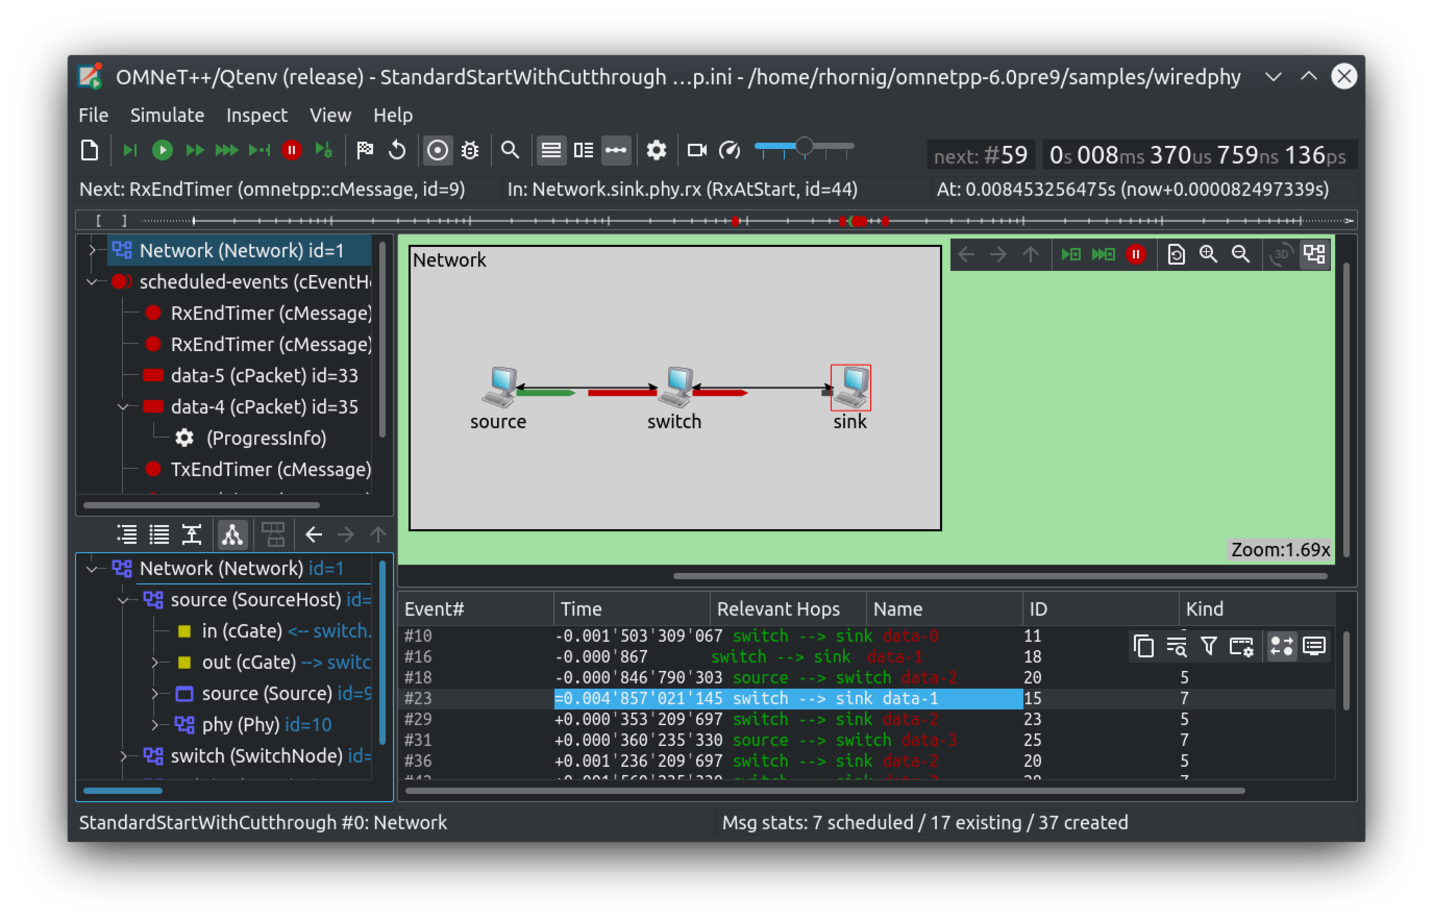
\includegraphics[width=0.75\textwidth]{parts/figuras/OMNET_IDE.pdf}
    \caption{A screenshot of the OMNET++ graphical interface from release 6. https://omnetpp.org/software/2020/11/03/omnet-6-pre9-released.html}
    \label{fig:OMNET_IDE}
\end{figure*}


Simu5G, on the other hand, is a library that extends the capabilities of the OMNeT++ simulator to model end-to-end behavior of 5G networks \cite{9211504}, including low latency, and high data rate communications. The library incorporates features such as dual connectivity, service-based architecture, and a wide variety of deployment scenarios from dense urban to rural settings, all within the scenario-based modeling provided by the OMNeT++ framework.

It specifically simulates the data plane of the 5G RAN (Release 16) and the core network. The library allows for simulation in both Frequency Division Duplexing (FDD) and Time Division Duplexing (TDD) modes across heterogeneous gNBs, ranging from macro to pico cell sizes, and it includes features such as handover support and inter-cell interference coordination via the X2 interface. 

Dual connectivity with LTE (eNB) and 5G NR (gNB) base stations is also supported, alongside 3GPP-compliant protocol layers. Realistic, customizable channel models are used for the physical layer, and the system supports resource scheduling in both uplink and downlink directions. Simu5G also supports numerous mobility models for user equipments, including those designed for vehicular mobility contexts.

